\documentclass[a4paper]{article}
%\documentclass[a4paper]{scrartcl}

\usepackage{url}
\usepackage{amsfonts}
\usepackage{amsmath}
\usepackage{amssymb}
\usepackage{subcaption}
\usepackage{float}
\usepackage{comment}
\usepackage{graphicx}
\usepackage{xcolor}

\renewcommand{\i}[1]{\textit{#1}}

\newcommand\blue[1]{\textcolor{blue}{#1}}

\newcommand{\judgmentdef}[2]{\fbox{#1}}
\newcommand{\inAnnLeftFrame}[1]{\isa{\_}{#1}}
\newcommand{\inRunFrame}{\run{\_}}
\newcommand{\inFixFrame}[2]{\fix{#1}{\_}{#2}}
\newcommand{\inInstLeftFrame}[1]{\inst{\_}{#1}}
\newcommand{\inInstRightFrame}[1]{\inst{#1}{\_}}
\newcommand{\inWrapLeftFrame}[2]{\wrap{#1}{\_}{#2}}
\newcommand{\inWrapRightFrame}[2]{\wrap{#1}{#2}{\_}}
\newcommand{\inUnwrapFrame}{\unwrap{\_}}
\newcommand{\inLamLeftFrame}[2]{\lam{#1}{\_}{#2}}
\newcommand{\inAppLeftFrame}[1]{\app{\_}{#1}}
\newcommand{\inAppELeftFrame}[1]{\app{\_}{#1}}
\newcommand{\inAppRightFrame}[1]{\app{#1}{\_}}
\newcommand{\inAppERightFrame}[1]{\app{#1}{\_}}
\newcommand{\inConFrame}[3]{\con{#1}{#2 ~ \_ ~ #3}}
\newcommand{\inCaseFrame}[1]{\case{\_}{#1}}
\newcommand{\inSuccessFrame}{\success{\_}}
\newcommand{\inBindFrame}[2]{\bind{\_}{#1}{#2}}
\newcommand{\inBuiltinFrame}[3]{\con{#1}{#2 ~ \_ ~ #3}}

\newcommand{\compute}{\mathrel\triangleright}
\newcommand{\return}{\mathrel\triangleleft}
\newcommand{\bcompute}{\color{blue}\compute}  
\newcommand{\breturn}{\color{blue}\return}  
\newcommand{\bmapsto}{\color{blue}\mapsto}
% This is to get blue symbols after an '&' inside an alignat environment.  It seems to mess up the spacing if you do anything else.


\newcommand{\ckerror}{\blacklozenge}


\newcommand{\construct}[1]{\texttt{(} #1 \texttt{)}}
\newcommand{\keyword}[1]{\texttt{#1}}

\newcommand{\repetition}[1]{\overline{#1}}
\newcommand{\unrepetition}[1]{\underline{#1}}

\newcommand{\inBuiltin}[5]{\builtin{#1}{#2}{#3\; #4\; #5}}

\newcommand{\builtin}[3]{\construct{\keyword{builtin} ~ #1 ~ #2 ~ #3}}
\newcommand{\con}[1]{\construct{\keyword{con} ~ #1}}
\newcommand{\abs}[3]{\construct{\keyword{abs} ~ #1 ~ #2 ~ #3}}
\newcommand{\inst}[2]{\texttt{\{}#1 ~ #2\texttt{\}}}
\newcommand{\lam}[3]{\construct{\keyword{lam} ~ #1 ~ #2 ~ #3}}
\newcommand{\lamE}[2]{\construct{\keyword{lam} ~ #1 ~ #2}}
\newcommand{\app}[2]{\texttt{[} #1 ~ #2 \texttt{]}}
\newcommand{\appE}[2]{\texttt{[} #1 ~ #2 \texttt{]}}
\newcommand{\fix}[3]{\construct{\keyword{fix} ~ #1 ~ #2 ~ #3}}
\newcommand{\run}[1]{\construct{\keyword{run} ~ #1}}
\newcommand{\fixE}[2]{\construct{\keyword{fix} ~ #1 ~ #2}}
\newcommand{\wrap}[3]{\construct{\keyword{wrap} ~ #1 ~ #2 ~ #3}}
\newcommand{\unwrap}[1]{\construct{\keyword{unwrap} ~ #1}}

\newcommand{\error}[1]{\construct{\keyword{error} ~ #1}}


\newcommand{\subst}[3]{[#1/#2]#3}
\newcommand{\substmulti}[2]{[#1]#2}


\author{Kenneth MacKenzie}
\date{November 2018}
\title{Lazy Evaluation and Plutus Core}
\begin{document}
\maketitle
\section{Introduction}
This document contains a description of a simple lazy abstract machine
for evaluation of Plutus Core.  For ease of comparison, it also
contains descriptions of the strict CK and CEK machines; there's also
a proposal for a (currently unimplemented) machine providing
constructs for both lazy and strict evaluation
(\S\ref{sec:strict-lazy}).  I've run the various machines on a
number of basic benchmarks, and \S\ref{sec:benchmarks} compares
the results and discusses the implications for the different
evaluation strategies.

The machines are described in the style of the Plutus Core
specification, in which a machine alternates between two main phases:
\textit{computation} ($\triangleright$), where it recurses down the
AST looking for values, saving surrounding contexts as frames (or
\textit{reduction contexts}) on a stack as it goes; and
\textit{return} ($\triangleleft$), where it has obtained a value and
pops a frame off the stack to tell it how to proceed next.  In
addition there is an error state $\blacklozenge$ which halts execution
with an error, and a stop state $\square$ which halts execution and
returns a value to the outside world. 

The presentation has been simplified slightly. For example, the
evaluators now take a table of dynamic built-in functions as a
parameter: we've omitted this because it's effectively a global
variable that's only used when calling builtins.

The machine states include various structures such as stacks,
environments, and heaps.  We will represent all of these by lists
which grow to the right; the symbol $\cdot$ denotes an empty
structure.  Looking something up in any of these structures always
proceeds from right to left, looking at most recent entries first.
(Note: the implementations don't necessarily use lists.)

Programs \texttt{(program \_ M)} are evaluated by evaluating the body
\texttt{M} in a state containing an empty stack (and an empty environment
and heap, if applicable).
 


\section{The CK Machine}
The CK machine originates in~\cite{Felleisen-Cek}, as does the CEK
machine.  The Plutus Core specification extends the basic CK machine
to cover all of Plutus Core, and this machine is (more or less)
reproduced in Figure~\ref{fig:ck-machine}.  This is based on version
5.3 of the Plutus Core specification.

%Note that all of our machines ignore types: specifically,
%evaluation of a type instantiation \texttt{\{M A\}} 

\newpage

%%% ---------------- CK machine ---------------- %%%
\begin{figure}[!ht]
\caption{The CK machine}\label{fig:ck-machine}
\centering
\begin{subfigure}[c]{\linewidth}  %% ---------------- CK machine states ---------------- %%
{\small
\caption{States}
    \[\begin{array}{lrclr}
        \textrm{Stack} & s      & ::= & f^*                               & \textrm{stacks}\\
        \textrm{State} & \sigma & ::= & s \compute M                  & \textrm{computing a term}\\
                       &        &     & s \return V                 & \textrm{returning a term value}\\
                       &        &     & \ckerror{}                        & \textrm{throwing an error}\\
                       &        &     & \square V                        & \textrm{halt and return a value}


    \end{array}\]
}
\end{subfigure}

\vspace{3mm}
\hrule
\vspace{3mm}

\begin{subfigure}[c]{\linewidth}      %% ---------------- CK machine frames ---------------- %%
{\small
\caption{Reduction frames}
\[
    \begin{array}{rlr}
      f ::= & \inInstLeftFrame{A}                     & \textrm{left instantiation}\\
            & \inWrapRightFrame{\alpha}{A}            & \textrm{right wrap}\\
            & \inUnwrapFrame{}                        & \textrm{unwrap}\\
            & \inAppLeftFrame{M}                      & \textrm{left application}\\
            & \inAppRightFrame{V}                     & \textrm{right application}\\
            & \inBuiltin{bn}{A^*}{V^*}{\_}{M^*}        & \textrm{builtin}\\
    \end{array}
\]
}
\end{subfigure}
\vspace{3mm}
\hrule
\vspace{3mm}

\begin{subfigure}[c]{\linewidth}   %% ---------------- CK machine ---------------- %%
{\small
\caption{Transitions}
     \begin{alignat*}{2}
      s &\compute \con{cn}                 &{}\mapsto{}& s \return \con{cn}\\
      s &\compute \abs{\alpha}{K}{M}       &{}\mapsto{}& s \return \abs{\alpha}{K}{M}\\
      s &\compute \inst{M}{A}              &{}\mapsto{}& s,\inInstLeftFrame{A} \compute M\\
      s &\compute \wrap{\alpha}{A}{M}      &{}\mapsto{}& s,\inWrapRightFrame{\alpha}{A} \compute M\\
      s &\compute \unwrap{M}               &{}\mapsto{}& s,\inUnwrapFrame{} \compute M\\
      s &\compute \lam{x}{A}{M}            &{}\mapsto{}& s \return \lam{x}{A}{M}\\
      s &\compute \app{M}{N}               &{}\mapsto{}& s,\inAppLeftFrame{N} \compute M\\
      s &\compute \builtin{bn}{\repetition{A}}{} &{}\mapsto{}& 
                                      s \return U \quad (\textit{$bn$ computes on $\repetition{A}$ to $U$})\\
      s &\compute \builtin{bn}{\repetition{A}}{M \repetition{M}} &{}\mapsto{}& 
                                      s,\inBuiltin{bn}{\repetition{A}}{}{\_}{\repetition{M}} \compute {M}\\
      s &\compute \error{A} &{}\mapsto{}& \ckerror{}\\
      \cdot &\return V &{}\mapsto{}& \square V\\
      s,\inInstLeftFrame{A} &\return \abs{\alpha}{K}{M} &{}\mapsto{}& s \compute{M} \\
      s,\inWrapRightFrame{\alpha}{A} &\return V         &{}\mapsto{}& s \return \wrap{\alpha}{A}{V}\\
      s,\inUnwrapFrame{} &\return {\wrap{\alpha}{A}{V}} &{}\mapsto{}& s \return V\\
      s,\inAppLeftFrame{N} &\return V                   &{}\mapsto{}& s, \inAppRightFrame{V} \compute N\\
      s,\inAppRightFrame{\lam{x}{A}{M}} &\return V      &{}\mapsto{}& s \compute \subst{V}{x}{M}\\
      s,  \inBuiltin{bn}{\repetition{A}}{\repetition{V}}{\_}{M \repetition{M}} &\return V &{}\mapsto{}& s, \inBuiltin{bn}{\repetition{A}}{\repetition{V} V}{\_}{\repetition{M}} \compute M\\
      s,\inBuiltin{bn}{\repetition{A}}{\repetition{V}}{\_}{} &\return V &{}\mapsto{}& s \return W \quad (\textit{$bn$ computes on $\repetition{A}$ and $\repetition{V}V$ to $W$})\\
    \end{alignat*}
}
\end{subfigure}
\end{figure}




\newpage

%%% ---------------- CEK machine ---------------- %%%

\section{The CEK Machine}
The CK machine is inefficient because it performs substitution on the
AST: when it is evaluating an application $[(\lambda x.M)\, N]$, it
reduces $N$ to a value $V$, then replaces all occurrences of $x$ in
$M$ with $V$ to obtain a new term $M^\prime$, which it then evaluates.
This is expensive both in terms of time and space.  If there are
several occurrences of $x$ in $M$ then they will all be replaced by
$V$, which could itself be a large term.

The CEK machine avoids this by extending the state of the machine with
\textit{environments} mapping variable names to closures consisting of
terms paired with environments\footnote{In the implementation, names
  are supplied with unique integer IDs which make them unambiguous;
  the environments in fact map these IDs to closures.}.  When the
machine is evaluating $[(\lambda x.M)\, N]$ in an environment $\rho$ it
first evaluates $N$ in $\rho$ to produce a value $V$, then extends
$\rho$ with the mapping $x \mapsto (V,\rho)$ to obtain a new
environment $\rho^{\prime}$, then proceeds to evaluate $M$ in the
environment $\rho^\prime$: when any occurrences of $x$ are encountered,
the machine retrieves the value $V$ from the environment and proceeds
with evaluation as normal.  It is necessary to use closures because
values may now contain variable names, and we have to know what the
variables were bound to at the time when the value was created.


The CEK machine is described in Figure~\ref{fig:cek-machine} and
reflects the implementation in the Plutus repository at the start of
November 2018.  This is very similar to the CK machine, except that
(1) every rule now involves environments, (2) a new rule has been
added to deal with the evaluation of variables, and (3) the rule
involving lambda application has changed to replace substitution with
the use of an extended environment. The major changes are
highlighted in \blue{blue}.




\paragraph{Built-in functions.} The rules involving \texttt{(builtin $b$\ $A_1, \ldots, A_n$
  $M_1\ \ldots M_n'$)} are possibly not quite correct: this is because
the interface to built-in functions has not yet been finalised.
Currently the machine evaluates each $M_i$ to a value $V_i$ and then
evaluates $b\ V_1 \ldots V_n$, discarding any environments associated
with the $V_i$.  It has to do this because built-in functions don't
know about environments, only values; in fact, the current
implementation can only deal with built-in functions all of whose
arguments are primitive values (like integers or bytestrings), and
supplying a non-primitive term as an argument will cause an error.
The precise form of arguments to built-in functions has not yet been
finalised: eventually we may have to do something like supplying
closures $(V_i, \rho_i)$ and substituting the contents of each
$\rho_i$ into $V_i$ to obtain completely concrete terms before calling
$b$.  This would re-introduce the inefficiency of the CK machine, so
it may be necessary to restrict the precise form of values which are
allowed to be taken as arguments by built-in functions. Moreover the
fact that we now have dynamic built-in functions which can be extended
by other people means that any such restriction will have to become
part of the Plutus Core specification.  Another thing that should be
specified is what kind of terms built-in functions can
\textit{return}: should they always be values, or could you get a term
which can undergo further evaluation?

A similar issue occurs when the machine terminates: if it's been
successful it will have produced a term $M$ together with an
environment $\rho$, but if we just print out the term $M$ it may not
tell you everything you want to know.  For example, the machine might
return the term $\lambda x.t$ with $t$ bound to $\lambda y.y$.  Thus
$M$ is ``really'' $\lambda x.\lambda y.y$, but this isn't apparent
from the AST for $M$.  This could be an issue if the machine has to
return a value to some entity in the blockhain infrastructure.  


\begin{figure}[!ht]
\caption{The CEK Machine}\label{fig:cek-machine}

\begin{subfigure}[c]{\linewidth}        %%% ---------------- CEK machine states ---------------- %%%
{\small
\caption{States}
\[
\begin{array}{lrcl}
        \textrm{Stack} & s      & ::= & f^*    \\
 \blue{       \textrm{Environment}} & \rho, \tau & ::= & [x \mapsto V]^* \\
        \textrm{State} & \sigma & ::= & s;\rho \compute M \quad | \quad s;\rho \return V  \quad | \quad \ckerror{} \quad | \quad \square (V,\rho)
    \end{array}
\]
}
\end{subfigure}

\vspace{1mm}
\hrule
\vspace{2mm}

\begin{subfigure}[c]{\linewidth}  %%% ---------------- CEK machine frames ---------------- %%%
{\small
\caption{Reduction frames}
\[
    \begin{array}{rlr}
       f ::= & \inInstLeftFrame{A}                     & \textrm{left instantiation}\\
             & \inWrapRightFrame{\alpha}{A}            & \textrm{right wrap}\\
             & \inUnwrapFrame{}                        & \textrm{unwrap}\\
             & \inAppLeftFrame{(M,\rho)}                 & \textrm{left application}\\
             & \inAppRightFrame{(V,\rho)}                & \textrm{right application}\\
             & \inBuiltin{bn}{A^*}{V^*}{\_}{M^*}        & \textrm{builtin}\\
    \end{array}
\]
}
\end{subfigure}
\vspace{1mm}
\hrule
\vspace{2mm}
\begin{subfigure}[c]{\linewidth}  %%% ---------------- CEK machine transitions ---------------- %%%
{
\small
\caption{Transitions}
    \begin{alignat*}{2}
     \blue{s; \rho} &\bcompute \blue{x}          &{}\bmapsto{}&\blue{s;\tau \return V \quad (\rho[x] = (V,\tau))}\\  % New rule
% Continuing with tau worries me
      s; \rho &\compute \con{cn}                 &{}\mapsto{}& s;\rho \return \con{cn}\\
      s; \rho &\compute \abs{\alpha}{K}{V}       &{}\mapsto{}& s;\rho \return \abs{\alpha}{K}{V}\\
      s; \rho &\compute \inst{M}{A}              &{}\mapsto{}& s,\inInstLeftFrame{A};\rho \compute M\\
      s; \rho &\compute \wrap{\alpha}{A}{M}      &{}\mapsto{}& s,\inWrapRightFrame{\alpha}{A};\rho  \compute M\\ 
      s; \rho &\compute \unwrap{M}               &{}\mapsto{}& s,\inUnwrapFrame{};\rho  \compute M\\
      s; \rho &\compute \lam{x}{A}{M}            &{}\mapsto{}& s;\rho \return \lam{x}{A}{M}\\
      s; \rho &\compute \app{M}{N}               &{}\mapsto{}& s,\inAppLeftFrame{(N,\rho)};\rho \compute M\\
      s; \rho &\compute \builtin{bn}{\repetition{A}}{} &{}\mapsto{}& s;\rho \return U \quad (\textit{$bn$ computes on $\repetition{A}$ to $U$})\\
      s; \rho &\compute \builtin{bn}{\repetition{A}}{M \repetition{M}} &{}\mapsto{}& s,\inBuiltin{bn}{\repetition{A}}{}{\_}{\repetition{M}};\rho \compute M\\
      s; \rho &\compute \error{A} &{}\mapsto{}& \ckerror{}\\
      \cdot; \rho &\return V &{}\mapsto{}& \square (V, \rho)\\
      s,\inInstLeftFrame{A}; \rho &\return \abs{\alpha}{K}{M} &{}\mapsto{}& s;\rho \compute{M} \\
      s,\inWrapRightFrame{\alpha}{A}; \rho &\return V &{}\mapsto{}& s;\rho \return \wrap{\alpha}{A}{V}\\
      s,\inUnwrapFrame{}; \rho &\return \wrap{\alpha}{A}{V} &{}\mapsto{}& s;\rho \return V\\
      s,\inAppLeftFrame{(N,\rho^{\prime})}; \rho &\return V &{}\mapsto{}& s, \inAppRightFrame{(V,\rho)};\rho^{\prime} \compute N\\
      \blue{s,\inAppRightFrame{(\lam{x}{A}{M}, \rho^{\prime})}; \rho} &\breturn V &{}\bmapsto{}& \blue{s;\rho^{\prime}[x\mapsto (V,\rho)] \compute M}\\  %% Modified
      s,  \inBuiltin{bn}{\repetition{A}}{\repetition{V}}{\_}{M \repetition{M}}{}; \rho&\return V &{}\mapsto{}& s, \inBuiltin{bn}{\repetition{A}}{\repetition{V} V}{\_}{\repetition{M}};\rho \compute M\\
      s,\inBuiltin {bn} {\repetition{A}} {\repetition{V}}{\_}{}; \rho &\return V 
                                                &{}\mapsto{}& s;\rho \return W \quad (\textit{$bn$ computes on $\repetition{A}$ and $\repetition{V}V$ to $W$})\\
\end{alignat*}
}
\end{subfigure}
\end{figure}


\begin{comment}
computeCek con (Apply _ fun arg)      = do
    varEnv <- getVarEnv
    computeCek (FrameApplyArg varEnv arg : con) fun
computeCek con (Var _ varName)        = do
computeCek con bi@Builtin{} = returnCek con bi

-- | The returning part of the CEK machine.
-- Returns 'EvaluationSuccess' in case the context is empty, otherwise pops up one frame
-- from the context and either
-- 1. performs reduction and calls 'computeCek' ('FrameTyInstArg', 'FrameApplyFun', 'FrameUnwrap')
-- 2. performs a constant application and calls 'returnCek' ('FrameTyInstArg', 'FrameApplyFun')
-- 3. puts 'FrameApplyFun' on top of the context and proceeds with the argument from 'FrameApplyArg'
-- 4. grows the resulting term ('FrameWrap')
returnCek :: Context -> Plain Value -> CekM EvaluationResult
returnCek []                                  res = pure $ EvaluationSuccess res
returnCek (FrameTyInstArg ty           : con) fun = instantiateEvaluate con ty fun
returnCek (FrameApplyArg argVarEnv arg : con) fun = do
    funVarEnv <- getVarEnv
    withVarEnv argVarEnv $ computeCek (FrameApplyFun funVarEnv fun : con) arg
returnCek (FrameApplyFun funVarEnv fun : con) arg = do
    argVarEnv <- getVarEnv
    applyEvaluate funVarEnv argVarEnv con fun arg
returnCek (FrameWrap ann tyn ty        : con) val = returnCek con $ Wrap ann tyn ty val
returnCek (FrameUnwrap                 : con) dat = case dat of
    Wrap _ _ _ term -> returnCek con term
    term            -> throwError $ MachineException NonWrapUnwrappedMachineError term

\end{comment}


\section{Krivine's Machine}
Our lazy machine is based on Krivine's machine~\cite{Krivine} which is
similar to the CK machine but instead implements a call-by-name
semantics.  As with the CEK machine, it uses environments, but now
mapping variable names to expressions (not values).  When it is
evaluating $[(\lambda x.M)\, N]$ it extends the current environment with
$[x \mapsto N]$ then immediately starts to evaluate the body $M$.  If
$x$ is encountered while evaluating $M$, the machine will look $x$ up,
obtaining $M$: it then evaluates $M$ to a value $V$ and continues with
the evaluation of $M$.  This strategy is clearly inefficient because
if $x$ occurs multiple times in $M$ then $N$ has to be re-evaluated
every time.

I haven't implemented the Krivine machine for Plutus Core or produced
a description of the extended machine that would be required; however,
this can easily be deduced from the lazy machine in the following
section.


\section{The L Machine}
Despite the Krivine machine's inefficiency, it has served as a basis
for many truly lazy machines (ie, machines with call-by-need
semantics rather than call-by-name): see ~\cite{Sestoft, Friedman,
  Douence}, for example.

I've implemented a simple lazy machine based on the L machine of Friedman
et al.~\cite{Friedman}.  The implementation closely follows the
implementation of the CEK machine.  The main change is that the
machine now manipulates closures instead of terms, and it introduces a
heap which is used to store arguments awaiting evaluation.  In more
detail:

\begin{itemize}
\item States now consist of a stack and a heap.
\item The machine uses closures $(M,\rho)$ instead of terms.  The CEK
  machine does this implicitly, but using explicit closures makes
  it easier to make sure that we're always using the correct
  environment to evaluate a term.  In addition, I'm not quite sure
  that the rule for evaluating variables $x$ in the CEK machine is
  correct.
\item The environment maps variables onto heap locations (these are
  just abstract positions in the heap: in the implementation they're
  Haskell Integers).
\item The heap contains closures which are tagged as being either
  \texttt{Unevaluated} or {Evaluated}.
\item When evaluation of an application $[(\lambda x.M)\, N]$ begins,
  the unevaluated term $N$ packaged into a closure $C$ along with the current
  environment, and $C$ is stored in the heap, tagged as 
  \texttt{Unevaluated}; the machine then goes on to evaluate $M$ in an
  environment with $x$ pointing to the location of $C$ in the heap.
\item When a reference to $x$ is encountered, the machine looks up $x$
  in the environment, obtaining a heap location $l$, and then looks up
  $l$ in the heap.  
  \begin{itemize} 
    \item If $l$ points to an \texttt{Unevaluated} closure $C = (N,
      \rho)$ (as will be the case the first time $x$ is seen) then the
      machine places an \texttt{update} marker on the stack and
      evaluates $N$ in the environment $\rho$ to obtain a closure $C^{\prime} =
      (V, \rho^{\prime})$; at this point the \texttt{update} marker
      will be back at the top of the stack and the heap is updated so
      that $l$ points to \texttt{Evaluated $C^{\prime}$}.  After this, the evaluation
      of $M$ continues with $C$ in place of $x$.
    \item If there are any later references to $x$, the machine will find
      the \texttt{Evaluated} closure $C^\prime$ and will be able to use it immediately.
  \end{itemize}
  \item Built-in functions don't know anything about laziness, so
    their arguments have to be evaluated before the function is
    called.  This is achieved as follows.  Suppose we have an
    application \texttt{($bn$ $M_1 \ldots M_n$)} (omitting types for
    simplicity). An appropriate \texttt{builtin} context containing
    the arguments $M_2, \ldots, M_n$ is placed on the stack and $M_1$ is
    evaluated to get a value $V_1$; the marker is popped off the stack to 
    obtain the remaining arguments, and a new \texttt{builtin} marker 
    containing $V_1,  M_3, \ldots, M_n$ is placed on the stack.  $M_2$ is
    then evaluated, and so on.  When all of the arguments have been evaluated
    to values, the function $bn$ is finally applied to them. 
    \begin{itemize}
      \item The issues mentioned earlier (in connection with the CEK
        machine) about the precise form of arguments to built in
        functions still obtain here.  The present implementation
        performs lazy evaluation to reduce arguments to values, so
        arguments may still contain pointers into the heap.  To avoid
        this we'd probably have to do a sort of deep forcing of the
        arguments; again, we can't make a decision about this right now.
      \item The strategy followed in the implementation is actually slightly different
        because the interface to built-in functions is in flux at the moment; however
        the effect is the same.
    \end{itemize}
  \item The heap is implemented as an integer counter together with a
    Haskell \texttt{IntMap} from integer locations to closures,
    When a new entry is inserted in the heap, the counter
    is incremented and used as a fresh heap location, and is returned 
    to the calling code for use in environments.
  \item The heap grows monotonically with no garbage collection or space re-use;
    the evaluation rules ensure that the current state of the heap is propagated 
    through the entire evaluation process.
    
\end{itemize}

%\newpage
%%% ---------------- L machine ---------------- %%%

\begin{figure}[!ht]
\caption{The L Machine}
\begin{subfigure}[c]{\linewidth}   %%% ---------------- L machine states ---------------- %%%
{\small
\caption*{(a) States}
\[
\begin{array}{lrcl}
        \textrm{Stack}           & s      & ::= & f^*\\
 \blue{ \textrm{Heap locations}} & l      &  & \\
 \blue{ \textrm{Heap entries}}   & e      & ::= & \texttt{Unevaluated } (M, \rho)\quad|\quad\texttt{Evaluated } (V,\rho) \\
 \blue{ \textrm{Environment}}    & \rho   & ::= & [x \mapsto l]^*\\
 \blue{ \textrm{Heap}}           & h      & ::= & [l \mapsto e]^*\\
        \textrm{State}           & \sigma & ::= & s;h \compute (M,\rho) \quad| \quad s;h \return (V, \rho)  \quad| \quad \ckerror{} \quad|\quad \square (V,\rho,h)
    \end{array}
\]
}
\end{subfigure}
\end{figure}
\begin{figure}

\begin{subfigure}[c]{\linewidth}     %%% ---------------- L machine frames ---------------- %%%
{
\small
\caption*{(b) Reduction frames}
\[
    \begin{array}{rlr}
      f :: = & \inInstLeftFrame{A}                     & \textrm{left instantiation}\\
             & \inWrapRightFrame{\alpha}{A}            & \textrm{right wrap}\\
             & \inUnwrapFrame{}                        & \textrm{unwrap}\\
             & \inAppLeftFrame{M}                      & \textrm{left application}\\
             & \texttt{(builtin \textit{bn} $A^*\ V^*\_\ M^*; \rho$)}        & \textrm{builtin}\\
             & \blue{\texttt{(update\ $l$)}}                   & \textrm{\blue{heap update marker}}\\
    \end{array}
\]
}
\end{subfigure}

\vspace{3mm}
\hrule
\vspace{3mm}

\hspace{-25mm}\begin{subfigure}[c]{\linewidth}   %%% ---------------- L machine transitions ---------------- %%%
{
\small
\caption*{\hspace{50mm}(c) Transitions}
\begin{alignat*}{2}\\
      \blue{s;h} &\bcompute \blue{(x, \rho)}        &{}\bmapsto{}& \blue{s;h \return (V,\rho^{\prime})  \hspace{62pt} (h[\rho[x]] = \texttt{Evaluated}\; (V, \rho^{\prime}))}\\  %% New rule
      \blue{s;h} &\bcompute \blue{(x, \rho)}        &{}\bmapsto{}& \blue{s,\texttt{(update\ $l$)}; h \compute (M,\rho^{\prime}) \quad (h[\rho[x]] = \texttt{Unevaluated}\; (M,\rho^{\prime}))}\\  %% New rule
      s;h &\compute (\con{cn}, \rho)               &{}\mapsto{}& s;h \return (\con{cn}, \rho)\\
      s;h &\compute (\abs{\alpha}{K}{V}, \rho)      &{}\mapsto{}& s;h \return (\abs{\alpha}{K}{V}, \rho)\\
      s;h &\compute (\inst{M}{A}, \rho)             &{}\mapsto{}& s,\inInstLeftFrame{A}; h \compute (M,\rho)\\
      s;h &\compute (\wrap{\alpha}{A}{M}, \rho)     &{}\mapsto{}& s,\inWrapRightFrame{\alpha}{A};h \compute (M, \rho)\\
      s;h &\compute (\unwrap{M}, \rho)              &{}\mapsto{}& s, \inUnwrapFrame{};h \compute (M,\rho)\\
      s;h &\compute (\lam{x}{A}{M}, \rho)           &{}\mapsto{}& s;h \return (\lam{x}{A}{M}, \rho)\\
      s;h &\compute (\app{M}{N}, \rho)              &{}\mapsto{}& s,\inAppLeftFrame{(N, \rho)};h \compute (M,\rho)\\
      s;h &\compute (\builtin{bn}{\repetition{A}}{}, \rho) 
                                                    &{}\mapsto{}& s;h \return (U,\rho) \quad (\textit{$bn$ computes on $\repetition{A}$ to $U$})\\
      s;h &\compute (\builtin{bn}{\repetition{A}}{M \repetition{M}}, \rho) 
                                                    &{}\mapsto{}& s,\inBuiltin{bn}{\repetition{A}}{}{\_}{\repetition{M}; \rho};h \compute (M, \rho)\\
      s;h &\compute (\error{A}, \rho) &{}\mapsto{}& \ckerror{}\\
      \cdot;h &\return (V, \rho) &{}\mapsto{}& \square(V, \rho, h)\\
      s,\inInstLeftFrame{A};h &\return (\abs{\alpha}{K}{M},\rho) 
                                                    &{}\mapsto{}& s;h \compute (M,\rho) \\
      s,\inWrapRightFrame{\alpha}{A};h &\return (V, \rho) &{}\mapsto{}& s;h \return (\wrap{\alpha}{A}{V}, \rho)\\
      s,\inUnwrapFrame{};h &\return (\wrap{\alpha}{A}{V}, \rho) 
                                                    &{}\mapsto{}& s;h \return (V,\rho)\\
      \blue{s,\inAppLeftFrame{(N,\rho^{\prime})};h} & \breturn (\lam{x}{A}{M}, \rho) 
                                                    &{}\bmapsto{}& \blue{s;h[l\mapsto \texttt{Unevaluated}\;(N,\rho^{\prime})] \compute (M, \rho[x \mapsto l])}\\
      & & & \hspace{2cm}\blue{(\textit{$l$ a fresh heap location})}\\
      \blue{s, \texttt{(update\ $l$)}}  & \breturn (V, \rho)   &{}\bmapsto{}& \blue{s;h[l\mapsto \texttt{Evaluated}\;(V, \rho)] \return (V,\rho)}\\
      s, \inBuiltin{bn}{\repetition{A}}{\repetition{V}}{\_}{M \repetition{M}; \rho}{}; h &\return (V , \rho^{\prime})
                                                    &{}\mapsto{}& s, \inBuiltin{bn}{\repetition{A}}{\repetition{V} V}{\_}{\repetition{M}; \rho};h \compute (M, \rho)\\
      s,\inBuiltin {bn} {\repetition{A}} {\repetition{V}}{\_}{; \rho}; h &\return (V, \rho^{\prime}) 
                                                    &{}\mapsto{}& s;h \return (W, \rho) \quad 
                                                    (\textit{$bn$ computes on $\repetition{A}$ and $\repetition{V}V$ to $W$})\\
\end{alignat*}
}
\end{subfigure}

\end{figure}



\newpage

\section{A machine providing both strict and lazy evaluation}\label{sec:strict-lazy}
The CEK machine and the L machine are quite similar, and it should be
relatively straightforward to combine the two to produce a machine
supporting both strict and lazy evaluation\footnote{It's tempting to
  refer to this as \textit{sleazy evaluation}.}.
\\

\noindent The basic idea is as follows:
\begin{itemize}
\item The machine would provide two forms of application:
  \begin{itemize}
  \item \textit{Strict application}, denoted by $[M N]$
  \item \textit{Lazy application}, denoted by $\langle M N \rangle$
  \end{itemize}
  \item Machine states would consist of a stack, a heap, and an environment;
    the environment would now contain two types of entry:
  \begin{itemize}
  \item \texttt{Strict} entries mapping names onto values.
  \item \texttt{Lazy} entries, mapping names onto heap locations.
  \end{itemize}
  \item To evaluate $[(\lambda x.M)\, N]$, $N$ would be evaluated immediately
    to obtain a value $V$ and the current environment would be extended to
    contain a \texttt{Strict} entry $[x \mapsto V]$.
  \item To evaluate $\langle (\lambda x.M)\, N \rangle$, a closure
    containing $N$ would be stored in the heap at some new location
    $l$ and environment would be extended to contain a \texttt{Lazy}
    entry $[x \mapsto l]$.
  \item Evaluation of names would then proceed in the obvious way:
    \texttt{Strict} entries would be used immediately and \texttt{Lazy}
    entries would be evaluated as in the L machine.
\end{itemize}


\noindent The obvious problem here is that if we want to perform a
strict application $[M N]$ then $N$ might contain lazy variables; for
example, we might have $N = \langle P\, Q \rangle$.  Presumably the
solution to this would be to introduce an operation to force all of
the lazy variables in $N$, analogous to Haskell's \texttt{deepseq}.
In the blockchain context, a possible problem with this approach (and
also with laziness in general) is that forcing a term with many lazy
subterms could cause a sudden large spike in gas consumption which
might not be expected by the user.




\section{Benchmarking}\label{sec:benchmarks}
I ran several simple benchmarks on each machine. These were all hand-coded
in Plutus Core, using the Z combinator for recursion; for the L machine, I also
had versions using the Y combinator (programs using this don't terminate on the 
strict machines).  There were four examples: Haskell versions are given below, 
together with comments.

\paragraph{Loop}
\begin{verbatim}
loop n = if n <= 0 then 0 else loop (n-1)
\end{verbatim}

\noindent This just makes $n$ recursive calls and then returns.
Running this gives some idea of the time and memory consumption
required by basic control structures like branching and recursion.

\paragraph{Triangular numbers}
\begin{verbatim}
tri n = if n <= 0 then 0 else n + tri (n-1)
\end{verbatim}

\noindent This calculates $n + (n-1) + \ldots + 2 + 1$.  This is equal to
$n(n-1)/2$, so we can perform quite a lot of recursion without using too much memory.

\paragraph{Factorial}
\begin{verbatim}
fac n = if n <= 0 then 1 else n * fac (n-1)
\end{verbatim}

\noindent As usual, this calculates $n(n-1)\cdots1$.  This is quickly
becomes very large, so we have to run this program with (perhaps
unrealistically) large sizes of integer.  Any differences between the
various machines are likely to be due to the evaluation mechanism.

\paragraph{Fibonacci}
\begin{verbatim}
fib n = if n <= 1 then 1 else fib(n-1) +  fib(n-2)
\end{verbatim}

\noindent This naive implementation performs a huge amount of
recursion (essentially \texttt{fib n} recursive calls) but relatively
little computation.

\subsection{Results}

\noindent The programs were run with the inputs shown in Figure~\ref{fig:benchmark-inputs}

\begin{figure}[H]
\centering
\begin{tabular}{|l|r|r|r|r|} 
\hline
Program   & Minimum input & Step & Maximum input & Integer size (bytes) \\
\hline
\texttt{loop} & 0 & 20,000 & 1,000,000 & 4\\
\texttt{tri}  & 0 & 50,000 & 2,000,000 & 8\\
\texttt{fac}  & 0 & 5,000 & 100,000 & 190,000\\
\texttt{fib}  & 1 & 1 & 31 & 4 \\
\hline
\end{tabular}
\caption{Programs and inputs}\label{fig:benchmark-inputs}
\end{figure}

\noindent
I ran these on a laptop with 8GB of memory and an Intel Core i5-4200U
processor running Linux.  Each program was run once only with each
input; ideally I'd have taken the average over several executions, but
the results are pretty conclusive anyway.  I measured the execution
time using \texttt{/usr/bin/time -f "\%U \%S \%M"}, which returns the
user time, the system time and the ``maximum resident set size'',
which seems to be a reasonable measure of memory usage.
Figures~\ref{fig:loop-graphs}--\ref{fig:fib-graphs} contain graphs
plotting the time taken (user+system) against the input size, and also
memory usage against input size.  Figure~\ref{fig:maxheap} shows the
final size of the L machine's heap for the maximum input to each
program.

\newpage
\begin{figure}[H]
\centering 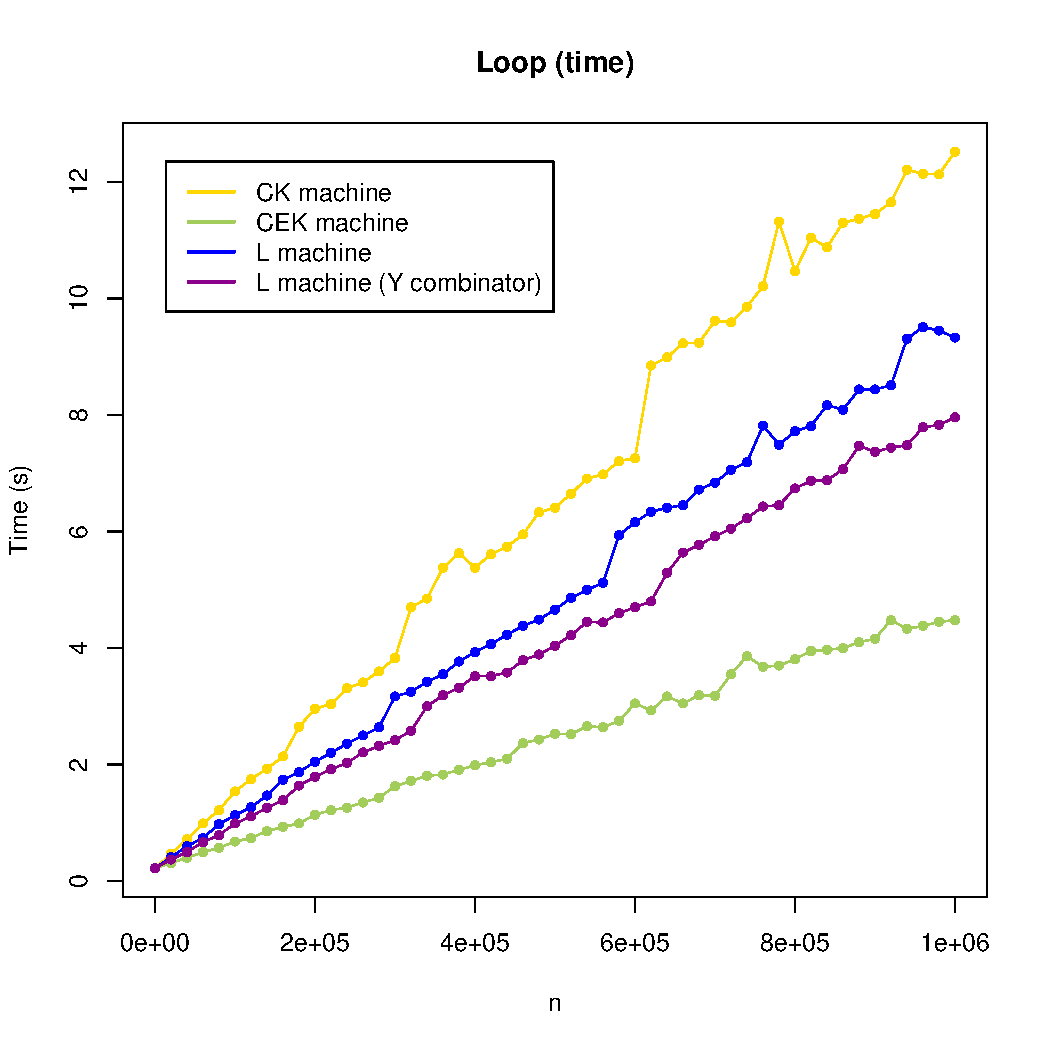
\includegraphics[width=0.7\linewidth]{figs/loop-times.pdf}

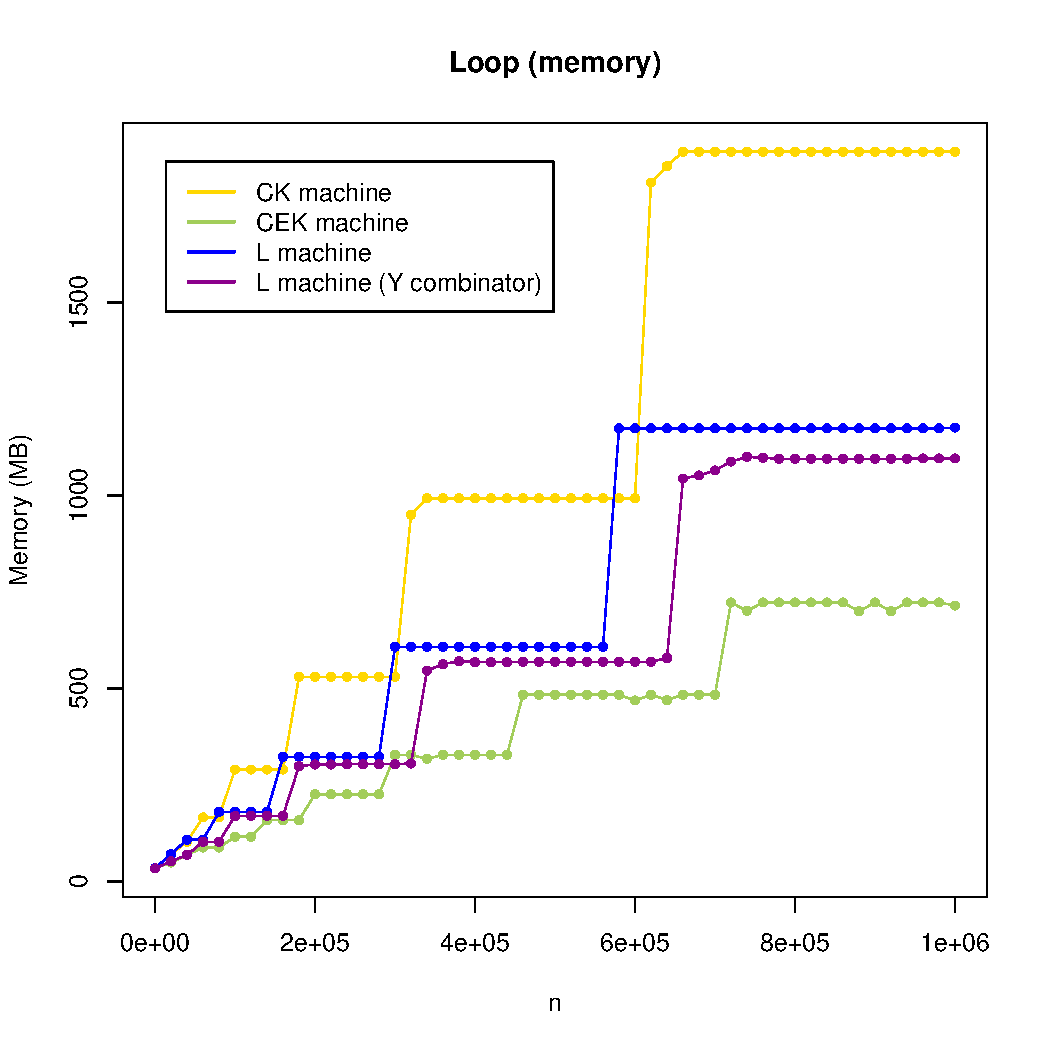
\includegraphics[width=0.7\linewidth]{figs/loop-mem.pdf}
\caption{Loop}\label{fig:loop-graphs}
\end{figure}
\newpage

\begin{figure}[H]
\centering
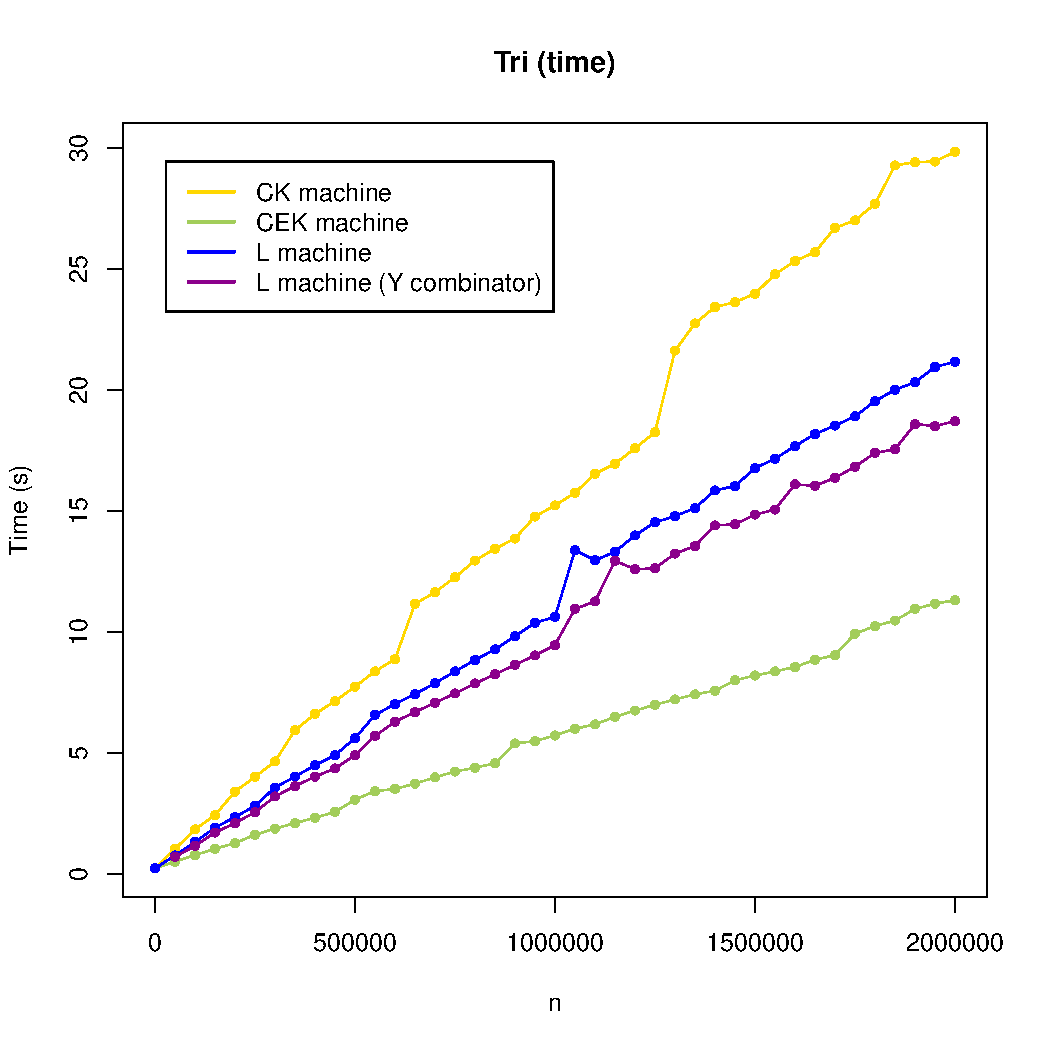
\includegraphics[width=0.7\linewidth]{figs/tri-times.pdf}

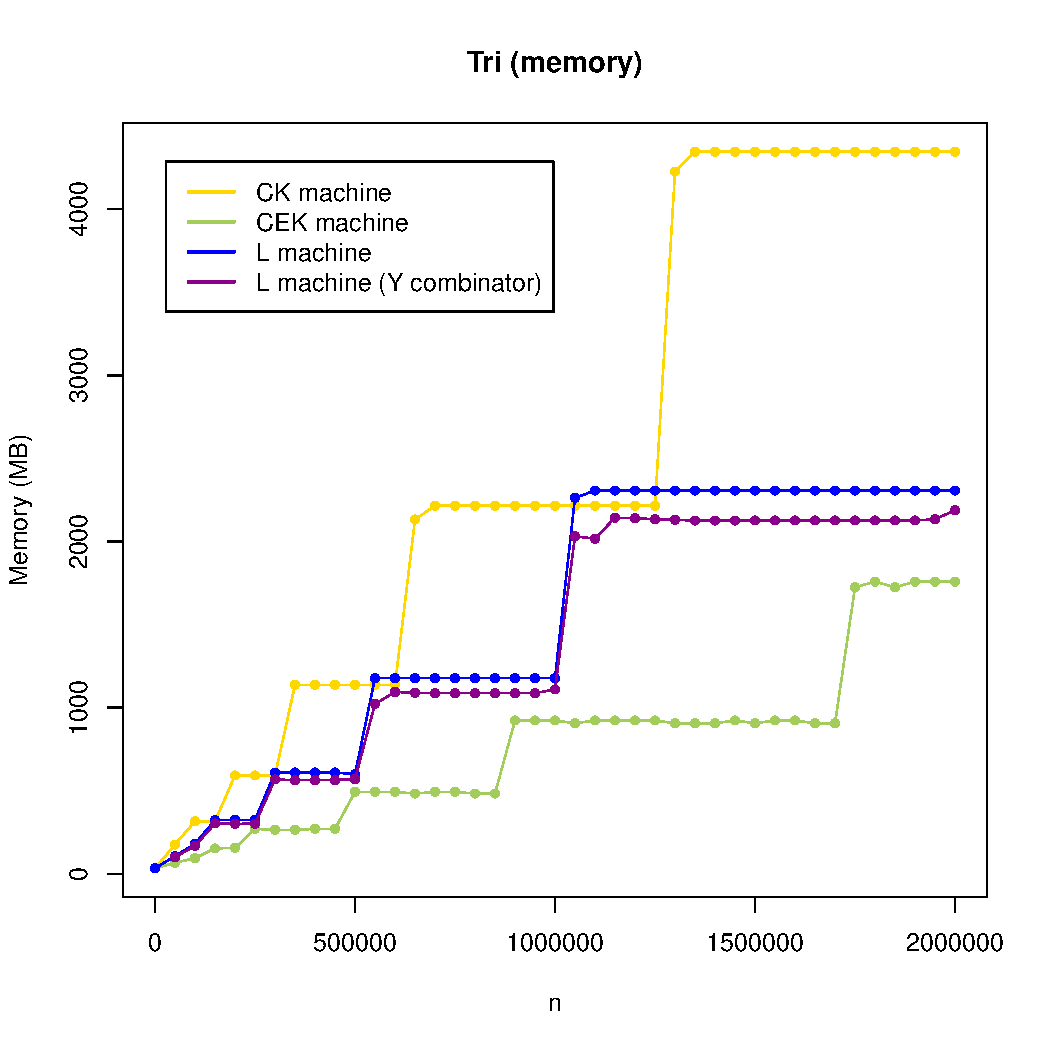
\includegraphics[width=0.7\linewidth]{figs/tri-mem.pdf}
\caption{Triangular numbers}\label{fig:tri-graphs}
\end{figure}
\newpage

\begin{figure}[H]
\centering
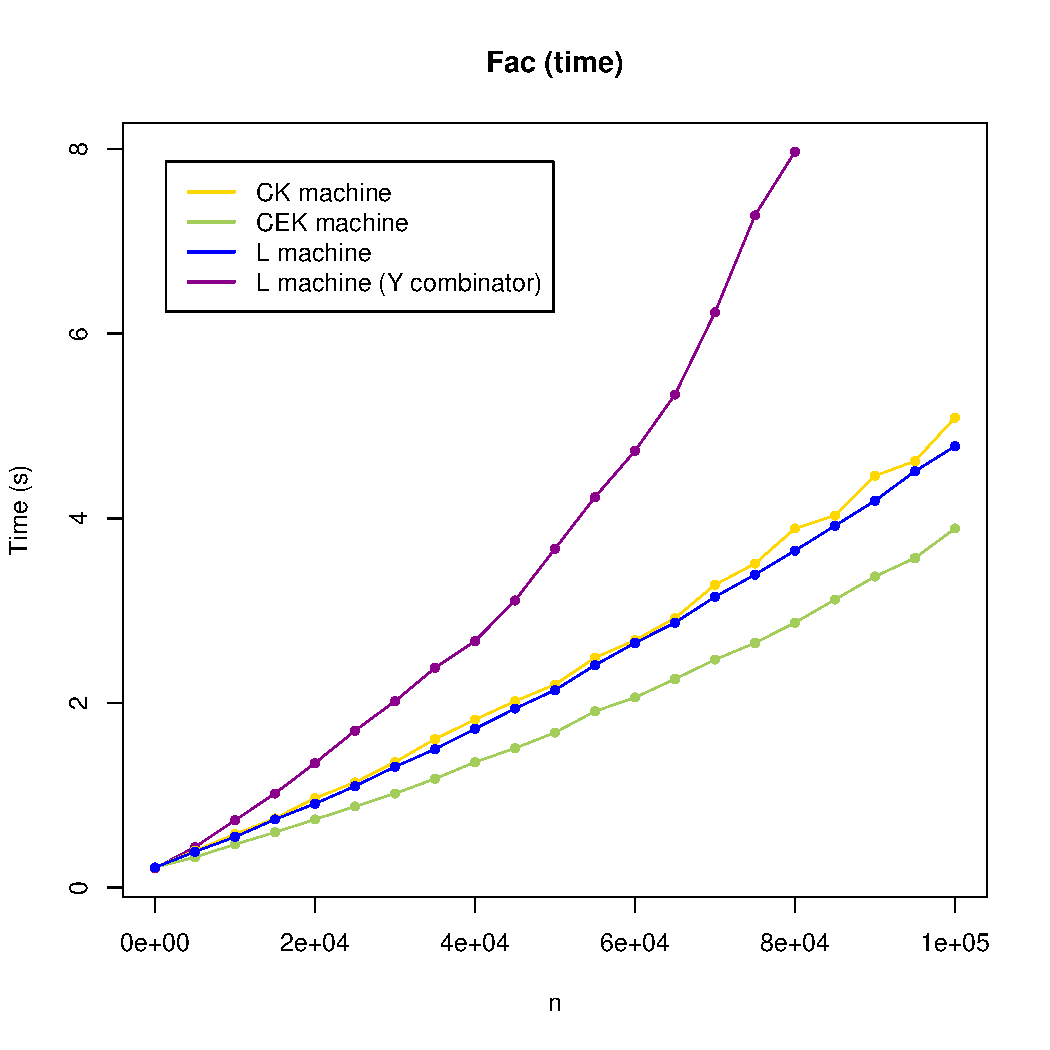
\includegraphics[width=0.7\linewidth]{figs/fac-times.pdf}
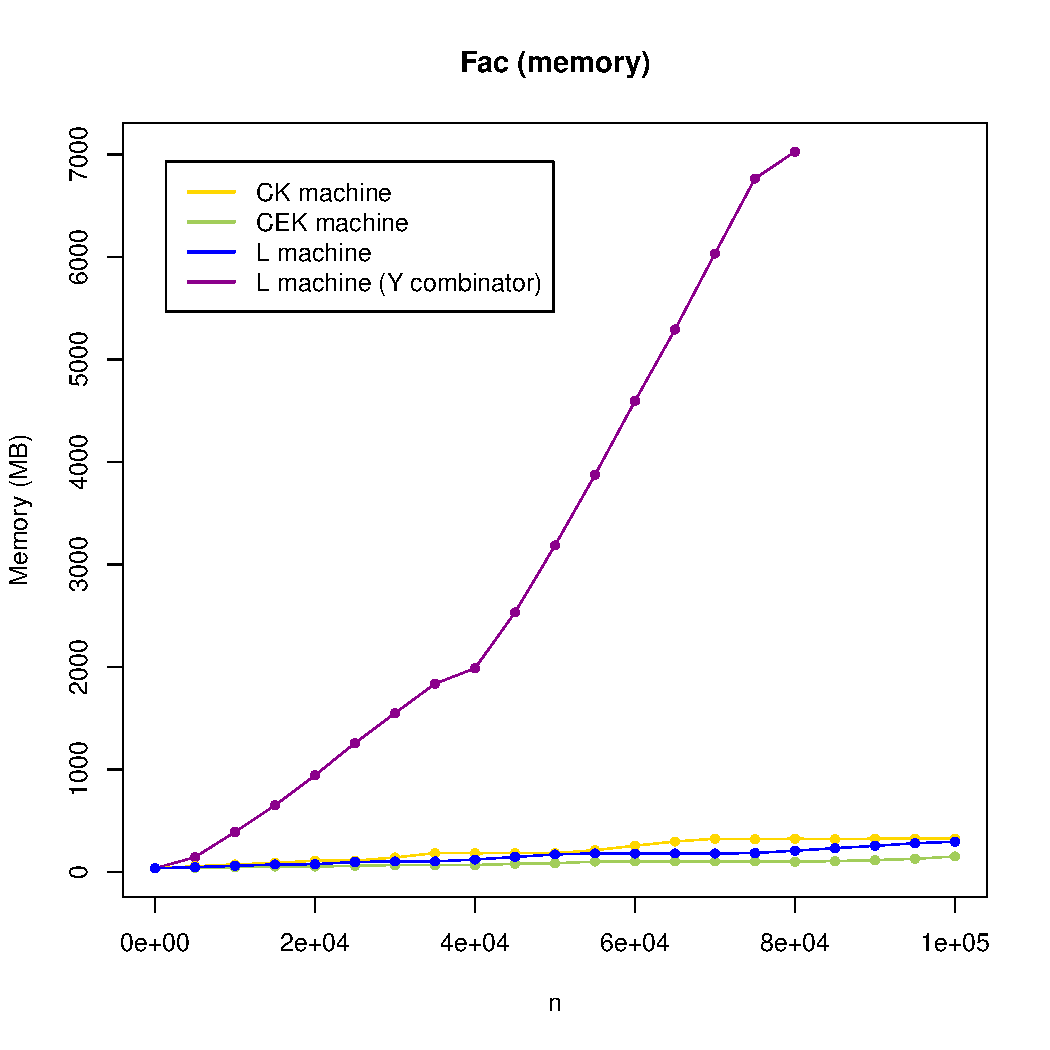
\includegraphics[width=0.7\linewidth]{figs/fac-mem.pdf}
\caption{Factorial}\label{fig:fac-graphs}
\end{figure}

\paragraph{Remarks.}  The version of factorial using the lazy machine and the Y-combinator 
ran out of memory at $n=85,000$ so no results appear for values beyond
that. Also, the memory graph ostensibly doesn't exhibit the step-like
behaviour seen in Figures~\ref{fig:loop-graphs} and
\ref{fig:tri-graphs}.  In fact the graph still looks like this for
small values of $n$, but it's not visible  because the scale's much more compressed.

\newpage
\begin{figure}[H]
\centering
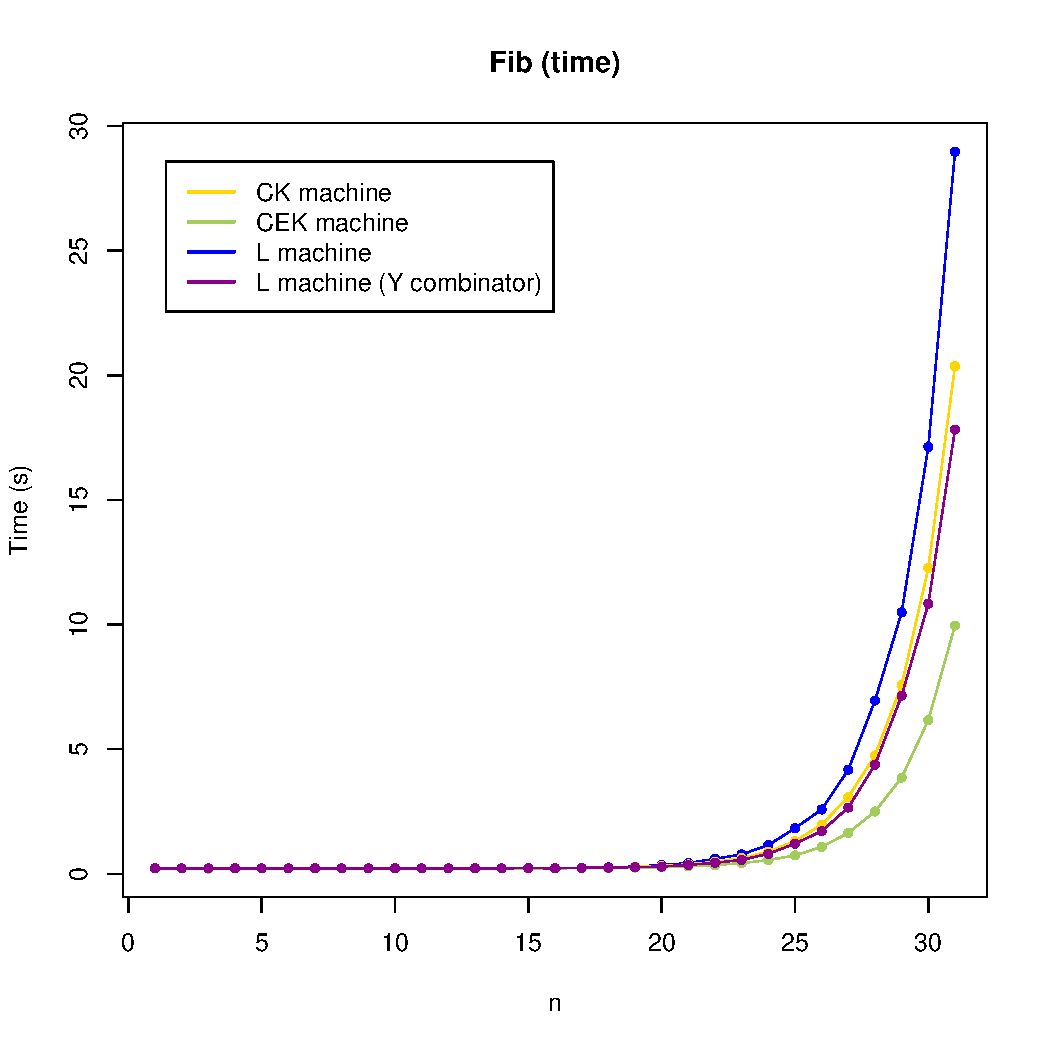
\includegraphics[width=0.7\linewidth]{figs/fib-times.pdf}
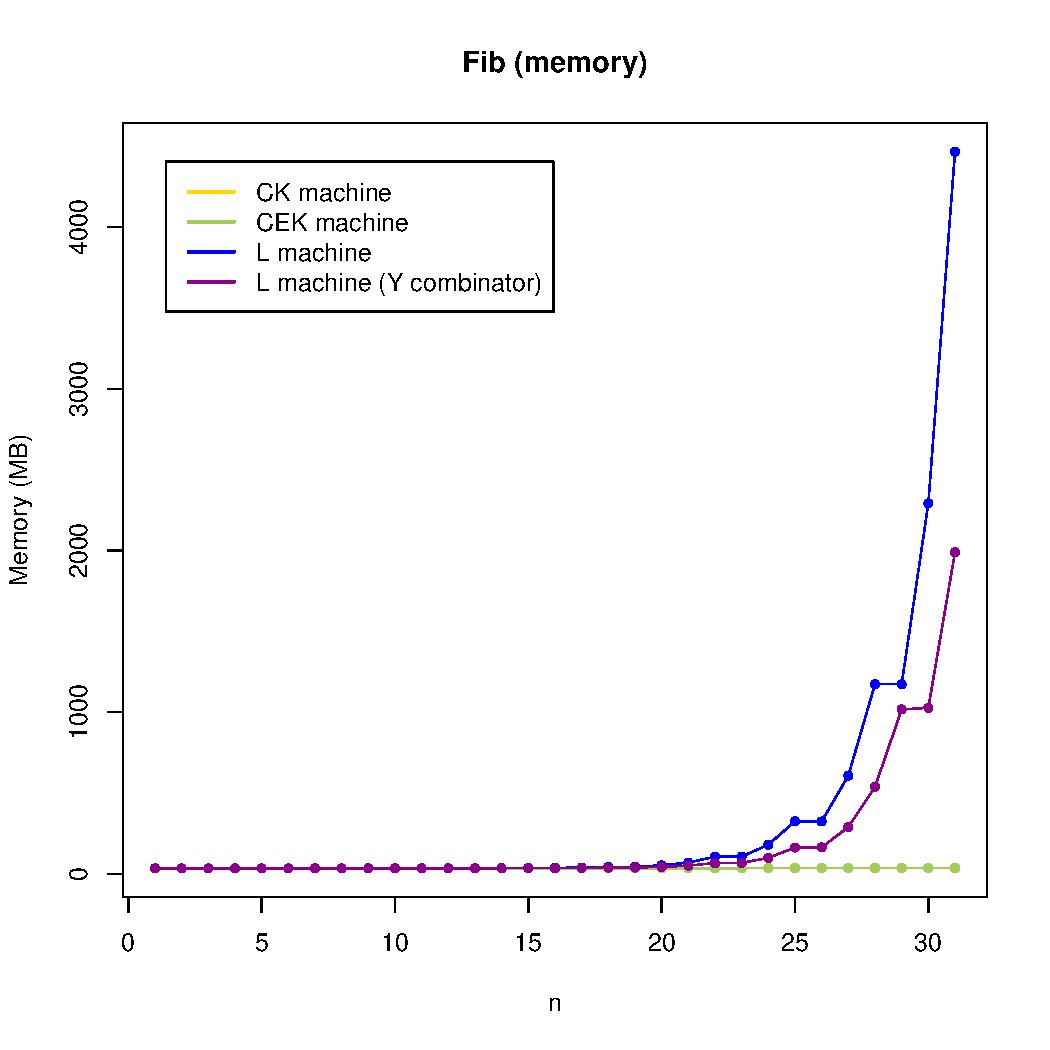
\includegraphics[width=0.7\linewidth]{figs/fib-mem.pdf}
\caption{Fibonacci}\label{fig:fib-graphs}
\end{figure}

\paragraph{Remarks.}  Again, the blocky nature of the memory usage is hidden because
of the scale.  The CK machine appears to be absent from the memory
graph, but it's hidden by the line for the CEK machine.
\newpage

\begin{figure}
\centering
\begin{tabular}{|l|r|r|r|r|} 
\hline
Program   &  Input &  Final heap size (cells) \\
\hline
\hline
\texttt{loop} (Z combinator) & 1,000,000 & 7,000,000\\
\texttt{loop} (Y combinator) & 1,000,000 & 5,000,001\\
\hline
\hline
\texttt{tri} (Z combinator)& 2,000,000 & 14,000,000\\
\texttt{tri} (Y combinator)& 2,000,000 & 10,000,001\\
\hline
\hline
\texttt{fac} (Z combinator)& 80,000 & 560,000 \\
\texttt{fac} (Y combinator)& 80,000 & 400,001\\
\hline
\hline
\texttt{fib} (Z combinator)& 31 & 18,847,759\\
\texttt{fib} (Y combinator)& 31 & 8,077,762\\
\hline
\end{tabular}
\caption{L machine heap size}\label{fig:maxheap}
\end{figure}


\subsection*{Discussion} It's clear that in all cases the CEK machine performs best, 
in terms both of time and memory.  The L machine with programs using
the Z combinator is always worse than the CEK machine but better than
the CK machine, except for \texttt{fib}.  For the Y combinator version
of \texttt{fac}, the memory usage is extremely bad, leading to
poor time performance as well.

It isn't surprising that the L machine is slower than the CEK machine.
When the CEK machine encounters a variable name $x$ it just has to
look up the already evaluated value of that variable in the current
environment.  In contrast, the L machine has to look up the heap
location $l$ corresponding to $x$, then look in the heap for the entry at $l$,
then look at whether the entry is \texttt{Evaluated} or
\texttt{Unevaluated} (and in the latter case evaluate it and modify the heap).
This adds an omnipresent overhead to variable accesses which is
unlikely to be recouped unless the program has many control paths
where arguments don't need to be evaluated (and note that built-in
functions \textit{always} have to have their arguments evaluated).
Admittedly, none of the programs used in these benchmarks
are sufficiently complex to allow any benefits of laziness to 
emerge.

The extremely poor behaviour of the L machine on the Y-combinator
version of the \texttt{fac} program is difficult to explain.
Observation of the size of the L machine's heap suggests that for
simple programs making $n$ recursive calls (like \texttt{loop},
\texttt{tri}, and \texttt{fac}), $7n$ cells are allocated if the Z
combinator is used, but only $5n+1$ for the Y combinator.  Thus the Y
version of \texttt{fac} uses \textit{less} memory in the machine's
internal heap than the Z version, and executes fewer machine
transitions, but is much slower and uses drastically more system
memory.  At the time of writing, I'm not sure what's going on,
especially in view of the fact that the \texttt{fac} program is
identical to the much better-behaved \texttt{tri} program, except that
\texttt{fac} is doing multiplication where \texttt{tri} is doing
addition.  It's conceivable that Haskell's laziness is interacting badly
with the L machine's evaluation strategy, but I don't have any
concrete evidence for that yet.  This program is highly unrealistic
though: it has to use integers of size 190,000 (which will take 185K
or more each if they're full up) to fit in the final answer (100,000!
has 456,574 digits); this will surely never be required in practice.

\section{Conclusions}
My feeling is that the CEK machine is probably almost optimal for
evaluation of Plutus Core programs.  The L machine adds an overhead
for every variable access, and has to access variable bindings through
an ever-growing heap.  Admittedly the L machine is about the simplest
possible lazy machine, and many improvements are possible:
see~\cite{Sestoft} and \cite{Friedman}, for example.  However, any
improvements will (a) add more overhead to the evaluation procedure,
and (b) complicate the evaluator (compare Figures 2 and 9
of~\cite{Friedman}), providing more opportunities for bugs to 
occur\footnote{
  One thing we might be able to do is eliminate the L
  machine's heap by allocating objects on Haskell's heap.
  Environments could map variable names to mutable reference cells in
  the Haskell heap containing \texttt{Unevaluated}/\texttt{Evaluated}
  objects which could be updated as required. This would save us from
  having to implement our own not-very-efficient heap and would give
  us garbage collection for free, but would make the Plutus Core
  semantics dependent on those of Haskell, which is probably
  undesirable.}.
Nonetheless, judicious use of laziness might permit some optimisation
by obviating the need to introduce explicit delays, eg, when
implementing fixpoint operators or branches.

I doubt that it's even possible to improve the CEK machine very much.
The simplicity of Plutus Core makes it very difficult to evaluate more
efficiently.  For example, the fact that every function takes exactly
one argument means that we have to introduce intermediate closures
when evaluating terms that are ``really'' $n$-ary applications.  Another
factor is that there are no easily-observable control structures which
could be handled specially by an evaluator.  Yet another factor is
than we can't afford to do much in the way of static analysis on-chain,
so we just have to evaluate code as it comes.

\subsection{More things to do}
The benchmarks that I've used here are clearly unrealistic, being very
simple; I've also had to use very large numbers to make the evaluator
run for long enough to get measurable results. The PlutusTX compiler
now seems to be able to handle highly complex programs, so it'd be
well worthwhile seeing how the various evaluators deal with such
things.  The benchmarking method (\texttt{/usr/bin/time}) is also
rather crude, so we should use the Haskell profiling system to see
what's really going on.  This would probably also help us to optimise
our implementations.



\bibliographystyle{plain} %% ... or whatever
\bibliography{lazy-plutus-core}
\end{document}
